\chapter{Quick Revision: PE-EC801B - Fiber Optic Communication}

This high-density revision sheet compiles core definitions, mathematical formulas, essential diagrams to practice drawing, frequently asked exam questions, and fast-recall points across all 6 units of the syllabus.


\section{Important Definitions}

\subsection{Unit I: Introduction}
\begin{itemize}
  \item   \textbf{Snell's Law:} A law stating that the ratio of the sines of the angles of incidence and refraction is equal to the ratio of velocities in the two media, or equivalently, the product of the refractive index and the sine of the angle is constant: $n_1 \sin \theta_1 = n_2 \sin \theta_2$.
  \item   \textbf{Critical Angle ($\theta_c$):} The minimum angle of incidence at the core-cladding boundary above which total internal reflection (TIR) occurs, defined as $\theta_c = \sin^{-1}(n_2/n_1)$.
  \item   \textbf{Acceptance Angle ($\theta_a$):} The maximum angle at which a ray of light entering the fiber core from air will be guided by total internal reflection along the fiber.
  \item   \textbf{Numerical Aperture (NA):} A dimensionless parameter measuring the light-gathering ability of the fiber, defined as the sine of the acceptance angle: $\text{NA} = \sin \theta_a = \sqrt{n_1^2 - n_2^2}$.
  \item   \textbf{Meridional Rays:} Rays of light that pass through the longitudinal axis of the fiber core, remaining within a single plane.
  \item   \textbf{Skew Rays:} Rays that propagate through the fiber core without crossing the fiber's central longitudinal axis, following a helical path.
\end{itemize}

\subsection{Unit II: Optical Fibers}
\begin{itemize}
  \item   \textbf{Normalized Frequency ($V$-number):} A dimensionless parameter that determines the number of guided modes a fiber can support: $V = \frac{2\pi a}{\lambda} \text{NA}$.
  \item   \textbf{Cutoff Wavelength ($\lambda_c$):} The minimum wavelength at which a single-mode fiber supports only the fundamental mode ($\text{LP}_{01}$), defined under the condition $V = 2.405$.
  \item   \textbf{Mode-Field Diameter (MFD):} A measure of the radial distribution of optical power in the fundamental mode of a single-mode fiber, representing the width where the intensity drops to $1/e^2$ of its peak.
  \item   \textbf{Step-Index Fiber:} A fiber with a constant refractive index in the core and a sudden decrease (step) at the core-cladding boundary.
  \item   \textbf{Graded-Index Fiber:} A fiber with a core refractive index that decreases continuously and parabolically from the center axis out to the cladding boundary.
\end{itemize}

\subsection{Unit III: Signal Degradation}
\begin{itemize}
  \item   \textbf{Attenuation:} The reduction in optical power of a signal as it propagates through a fiber, measured in $\text{dB/km}$.
  \item   \textbf{Dispersion:} The temporal broadening of an optical pulse as it travels along a fiber, limiting the transmission bandwidth.
  \item   \textbf{Intermodal Dispersion:} Pulse broadening in multimode fibers caused by different modes traveling at different group velocities, arriving at different times.
  \item   \textbf{Intramodal (Chromatic) Dispersion:} Pulse broadening within a single mode caused by different wavelength components traveling at different speeds, consisting of material and waveguide dispersion.
  \item   \textbf{Optical Time Domain Reflectometer (OTDR):} An instrument that injects high-power optical pulses into a fiber and measures the backscattered and reflected light (Rayleigh scattering and Fresnel reflection) to locate faults and measure attenuation.
  \item   \textbf{GRIN-rod Lens:} A compact graded-index glass cylinder where the refractive index decreases parabolically from the central axis, used for collimating or focusing light.
  \item   \textbf{Expanded-Beam Connector:} A fiber connector that uses lenses to expand and collimate the exiting beam across an air gap, reducing lateral alignment sensitivity.
\end{itemize}


\subsection{Unit IV: Optical Sources \& Detectors}
\begin{itemize}
  \item   \textbf{Population Inversion:} A state in a laser medium where more electrons reside in a higher, excited energy state than in a lower, ground state, enabling net optical amplification.
  \item   \textbf{Threshold Gain ($g_{th}$):} The minimum gain required in a laser cavity to balance the internal and mirror reflection losses, allowing laser oscillation to begin.
  \item   \textbf{Responsivity ($R$):} The ratio of generated photocurrent to the incident optical power in a photodetector, measured in $\text{A/W}$.
  \item   \textbf{Quantum Efficiency ($\eta$):} The ratio of the number of electron-hole pairs collected at the terminals of a photodetector to the number of incident photons.
  \item   \textbf{Avalanche Photodiode (APD):} A highly sensitive photodetector that uses impact ionization under high reverse bias to provide internal current gain through avalanche multiplication.
  \item   \textbf{Isotype \& Anisotype Heterojunctions:} Isotype is a junction between two different materials of the same conductivity type (e.g. n-N). Anisotype is between different conductivity types (e.g. p-N).
  \item   \textbf{Radiative Minority Carrier Lifetime ($\tau_r$):} The average time an injected minority carrier survives in a band before undergoing radiative recombination.
\end{itemize}


\subsection{Unit V: Optical Switches \& Amplifiers}
\begin{itemize}
  \item   \textbf{Erbium-Doped Fiber Amplifier (EDFA):} A lumped optical amplifier that uses Erbium ions embedded in a silica core, pumped at $980\text{ nm}$ or $1480\text{ nm}$, to amplify signals directly in the $1550\text{ nm}$ window.
  \item   \textbf{Raman Amplifier:} An amplifier that exploits Stimulated Raman Scattering (SRS) in the transmission fiber to transfer energy from high-power pump lasers to signal wavelengths distributed along the link.
  \item   \textbf{Coupling Length ($L_c$):} The physical length of a directional coupler required for $100\%$ of the optical power to transfer from the launch waveguide to the parallel waveguide.
  \item   \textbf{Wavelength Division Multiplexing (WDM):} The technique of combining multiple optical carrier signals of different wavelengths onto a single optical fiber to increase data capacity.
\end{itemize}

\subsection{Unit VI: Nonlinear Effects}
\begin{itemize}
  \item   \textbf{Kerr Effect:} The phenomenon where the refractive index of a medium changes in proportion to the local optical intensity of the propagating light: $n(I) = n_0 + n_2 I$.
  \item   \textbf{Self-Phase Modulation (SPM):} A nonlinear phase shift induced on an optical pulse by its own intensity envelope, leading to spectral broadening.
  \item   \textbf{Four-Wave Mixing (FWM):} A parametric nonlinear process where three waves of different frequencies beat together to generate new intermodulation sidebands.
  \item   \textbf{Optical Soliton:} A stable optical pulse that propagates over long distances without changing its shape, achieved by balancing anomalous Group Velocity Dispersion (GVD) and Self-Phase Modulation (SPM).
\end{itemize}


\section{Key Formulas}

\subsection{1. Numerical Aperture (NA) \& Acceptance Angle}
\[ \text{NA} = \sin \theta_a = \sqrt{n_1^2 - n_2^2} \approx n_1 \sqrt{2\Delta} \]
\[ \Delta = \frac{n_1 - n_2}{n_1} \]
\begin{itemize}
  \item   Where:
  \item   $\theta_a$ = Acceptance angle in air
  \item   $n_1$ = Core refractive index
  \item   $n_2$ = Cladding refractive index
  \item   $\Delta$ = Relative refractive index difference
\end{itemize}
\textit{   }Numerical Example:* Given $n_1 = 1.48$ and $n_2 = 1.46$:
    \[ \Delta = \frac{1.48 - 1.46}{1.48} \approx 0.0135 \]
    \[ \text{NA} = \sqrt{1.48^2 - 1.46^2} = \sqrt{2.1904 - 2.1316} \approx \mathbf{0.242} \]
    \[ \theta_a = \sin^{-1}(0.242) \approx \mathbf{14.0^\circ} \]

\subsection{2. Normalized Frequency ($V$-number) \& Mode Count ($N$)}
\[ V = \frac{2\pi a}{\lambda} \text{NA} \]
\[ N_{\text{step}} \approx \frac{V^2}{2} \quad \text{and} \quad N_{\text{graded}} \approx \frac{V^2}{4} \]
\begin{itemize}
  \item   Where:
  \item   $a$ = Core radius
  \item   $\lambda$ = Operating wavelength
  \item   $N_{\text{step}}, N_{\text{graded}}$ = Total number of guided modes
\end{itemize}
\textit{   }Numerical Example:* A step-index fiber with core diameter $80\ \mu\text{m}$ ($a = 40\ \mu\text{m}$), $\text{NA} = 0.2$, operating at $\lambda = 0.85\ \mu\text{m}$:
    \[ V = \frac{2\pi \times 40}{0.85} \times 0.2 \approx \mathbf{59.14} \]
    \[ N_{\text{step}} \approx \frac{59.14^2}{2} \approx \mathbf{1749 \text{ modes}} \]

\subsection{3. Cutoff Wavelength ($\lambda_c$) for Single-Mode Fiber}
\[ \lambda_c = \frac{2\pi a \text{NA}}{V_c} = \frac{2\pi a \text{NA}}{2.405} \]
\begin{itemize}
  \item   Where:
  \item   $V_c = 2.405$ is the single-mode cutoff limit.
\end{itemize}
\textit{   }Numerical Example:* For core radius $a = 4.5\ \mu\text{m}$ and $\text{NA} = 0.12$:
    \[ \lambda_c = \frac{2\pi \times 4.5 \times 0.12}{2.405} \approx \mathbf{1.409\ \mu\text{m}} = \mathbf{1409\text{ nm}} \]

\subsection{4. Attenuation Coefficient ($\alpha$)}
\[ \alpha_{\text{dB/km}} = \frac{10}{L} \log_{10}\left(\frac{P_{\text{in}}}{P_{\text{out}}}\right) \]
\begin{itemize}
  \item   Where:
  \item   $L$ = Fiber link length in $\text{km}$
  \item   $P_{\text{in}}$ = Optical power launched at input
  \item   $P_{\text{out}}$ = Optical power measured at output
\end{itemize}

\subsection{5. Multimode Intermodal Delay ($\Delta\tau$) \& RMS Broadening ($\sigma_{\text{inter}}$)}
\[ \Delta\tau = \frac{L n_1 \Delta}{c} \quad \text{and} \quad \sigma_{\text{inter}} \approx \frac{L n_1 \Delta}{2\sqrt{3}c} \]
\begin{itemize}
  \item   Where:
  \item   $c$ = Speed of light in vacuum ($\approx 3 \times 10^5\text{ km/s}$)
  \item   $\Delta\tau$ = Total delay difference between fastest and slowest modes.
\end{itemize}

\subsection{6. Photodetector Responsivity ($R$) \& Quantum Efficiency ($\eta$)}
\[ R = \frac{\eta q}{h \nu} = \frac{\eta q \lambda}{h c} \approx \frac{\eta \lambda}{1.24} \]
\begin{itemize}
  \item   Where:
  \item   $q$ = Electron charge ($1.6 \times 10^{-19}\ \text{C}$)
  \item   $h$ = Planck's constant ($6.626 \times 10^{-34}\ \text{J}\cdot\text{s}$)
  \item   $\lambda$ = Wavelength in $\mu\text{m}$
\end{itemize}
\textit{   }Numerical Example:* A photodiode operating at $\lambda = 1.3\ \mu\text{m}$ with quantum efficiency $\eta = 70\%$ ($0.7$):
    \[ R \approx \frac{0.7 \times 1.3}{1.24} \approx \mathbf{0.734\ \text{A/W}} \]

\subsection{7. Laser Cavity Dynamics and Physics Equations}
\begin{itemize}
  \item   \textbf{Facet Reflectivity ($R$):}
\end{itemize}
    \[ R = \left( \frac{n - 1}{n + 1} \right)^2 \]
    \textit{(where $n$ is refractive index of active semiconductor).}
\begin{itemize}
  \item   \textbf{Longitudinal Mode Count ($m$):}
\end{itemize}
    \[ m = \frac{2nL}{\lambda} \]
    \textit{(where $L$ is cavity length and $\lambda$ is free-space wavelength).}
\begin{itemize}
  \item   \textbf{Mode Frequency Separation ($\Delta f$):}
\end{itemize}
    \[ \Delta f = \frac{c}{2nL} \]
\begin{itemize}
  \item   \textbf{Mode Wavelength Separation ($\Delta \lambda$):}
\end{itemize}
    \[ \Delta \lambda = \frac{\lambda^2 \Delta f}{c} = \frac{\lambda^2}{2nL} \]
\begin{itemize}
  \item   \textbf{Radiative Minority Carrier Lifetime ($\tau_r$):}
\end{itemize}
    \[ \tau_r = \frac{1}{B \cdot p_0} \]
    \textit{(where $B$ is recombination coefficient and $p_0$ is majority carrier hole concentration).}


\subsection{7. Rise-Time Budget for Digital Links}
\[ t_{\text{sys}} = \sqrt{t_{\text{tx}}^2 + t_{\text{disp}}^2 + t_{\text{rx}}^2} \le 0.7 T \quad (\text{for NRZ coding}) \]
\begin{itemize}
  \item   Where:
  \item   $t_{\text{sys}}$ = Total system rise-time.
  \item   $t_{\text{tx}}, t_{\text{rx}}$ = Transmitter and receiver electrical rise-times.
  \item   $t_{\text{disp}}$ = Fiber dispersion rise-time (chromatic + modal).
  \item   $T$ = Bit period ($1/\text{BitRate}$).
\end{itemize}

\subsection{8. Directional Coupler Power Equations}
\[ P_1(z) = P_0 \cos^2(\kappa z) \quad \text{and} \quad P_2(z) = P_0 \sin^2(\kappa z) \]
\[ L_c = \frac{\pi}{2\kappa} \]
\begin{itemize}
  \item   Where:
  \item   $\kappa$ = Evanescent coupling coefficient
  \item   $L_c$ = Coupling length
\end{itemize}

\subsection{9. Soliton Peak Power ($P_0$)}
\[ P_0 = \frac{|\beta_2|}{\gamma T_0^2} \]
\begin{itemize}
  \item   Where:
  \item   $\beta_2$ = Group Velocity Dispersion (GVD) parameter ($\text{s}^2/\text{m}$)
  \item   $\gamma$ = Fiber nonlinearity coefficient ($\text{W}^{-1}\text{km}^{-1}$)
  \item   $T_0$ = Half-width (pulse duration parameter) of the soliton
\end{itemize}


\section{Diagrams to Practice Drawing}

Prepare to sketch these block architectures, ray paths, and schematic layouts by hand for long-form answers:

\subsection{1. General \& Fiber-Optic Communication Systems (Unit I)}
Detailed comparison of general electronic vs. photonic transmission pipelines.  
\begin{figure}[H]
\centering
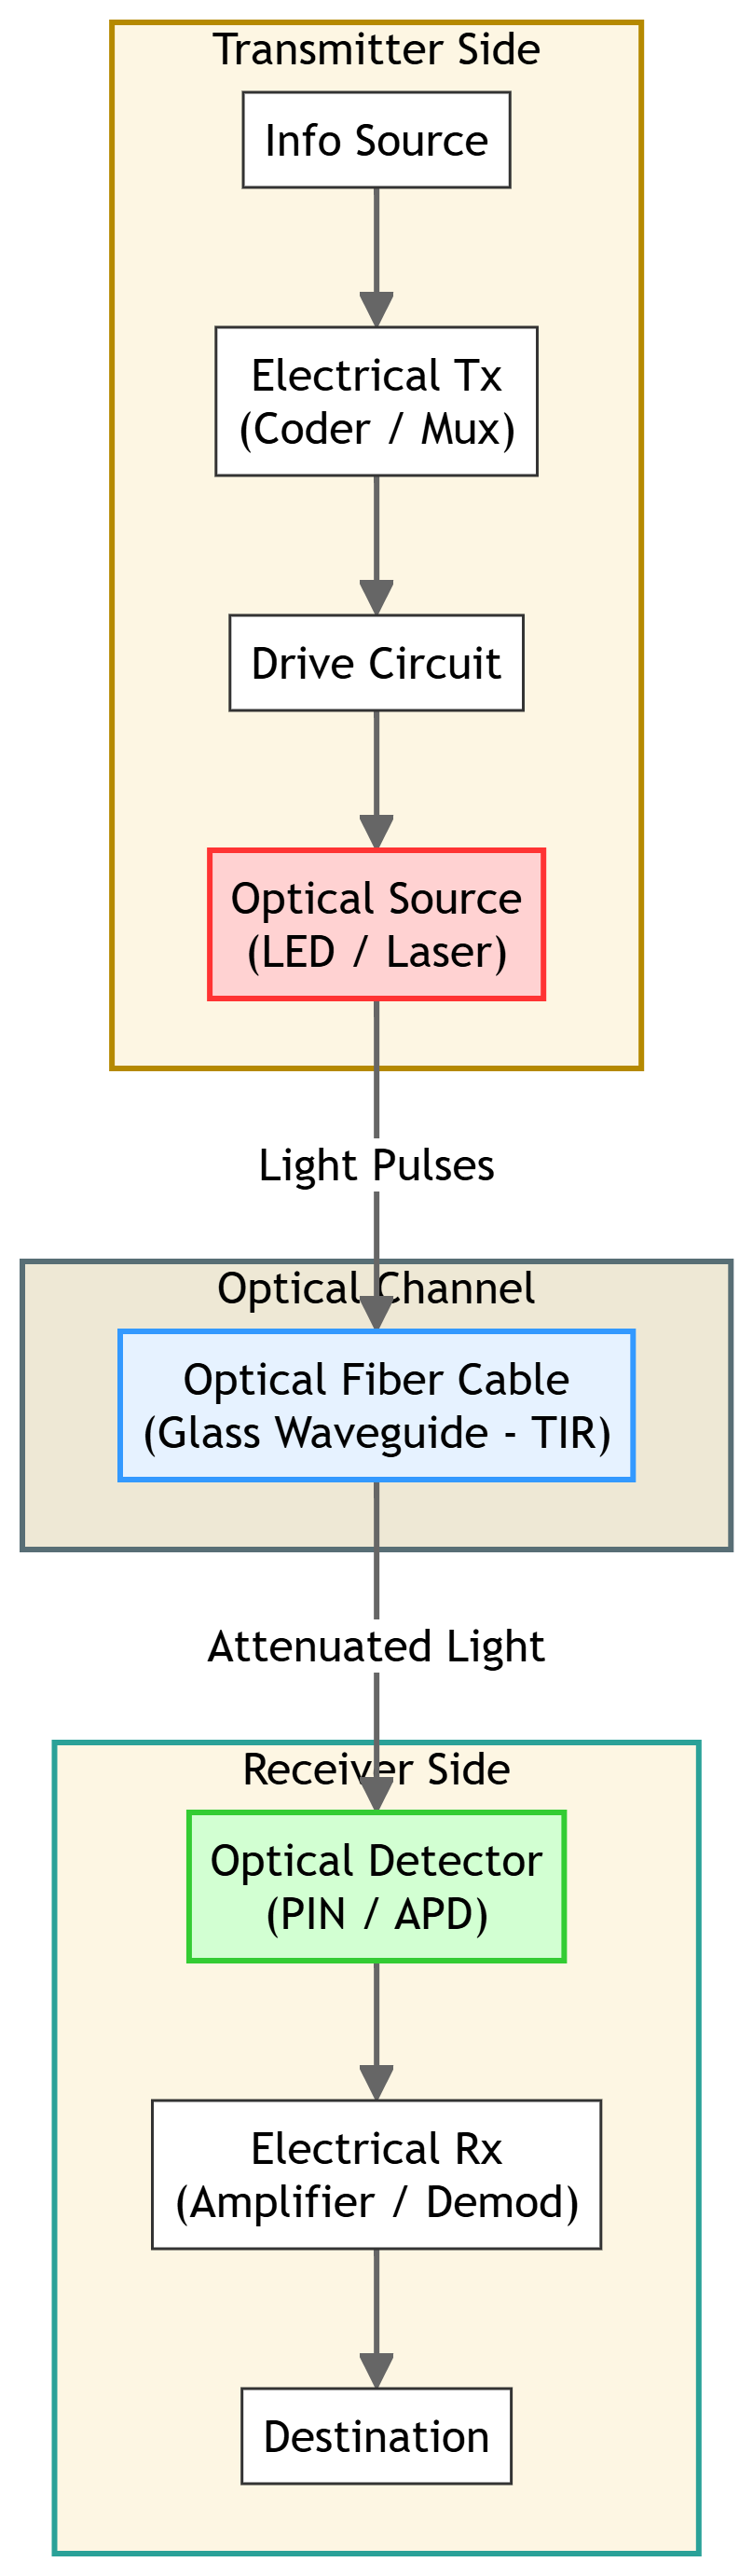
\includegraphics[width=0.75\textwidth,height=0.32\textheight,keepaspectratio]{../Images/chapter_01/fiber_comm_block.png}
\caption{General \& Fiber-Optic Communication System}
\end{figure}

\subsection{2. Ray Propagation \& Numerical Aperture (Unit I)}
Ray paths at the core-cladding boundary showing refraction, critical angle, and acceptance cone.  
\begin{figure}[H]
\centering
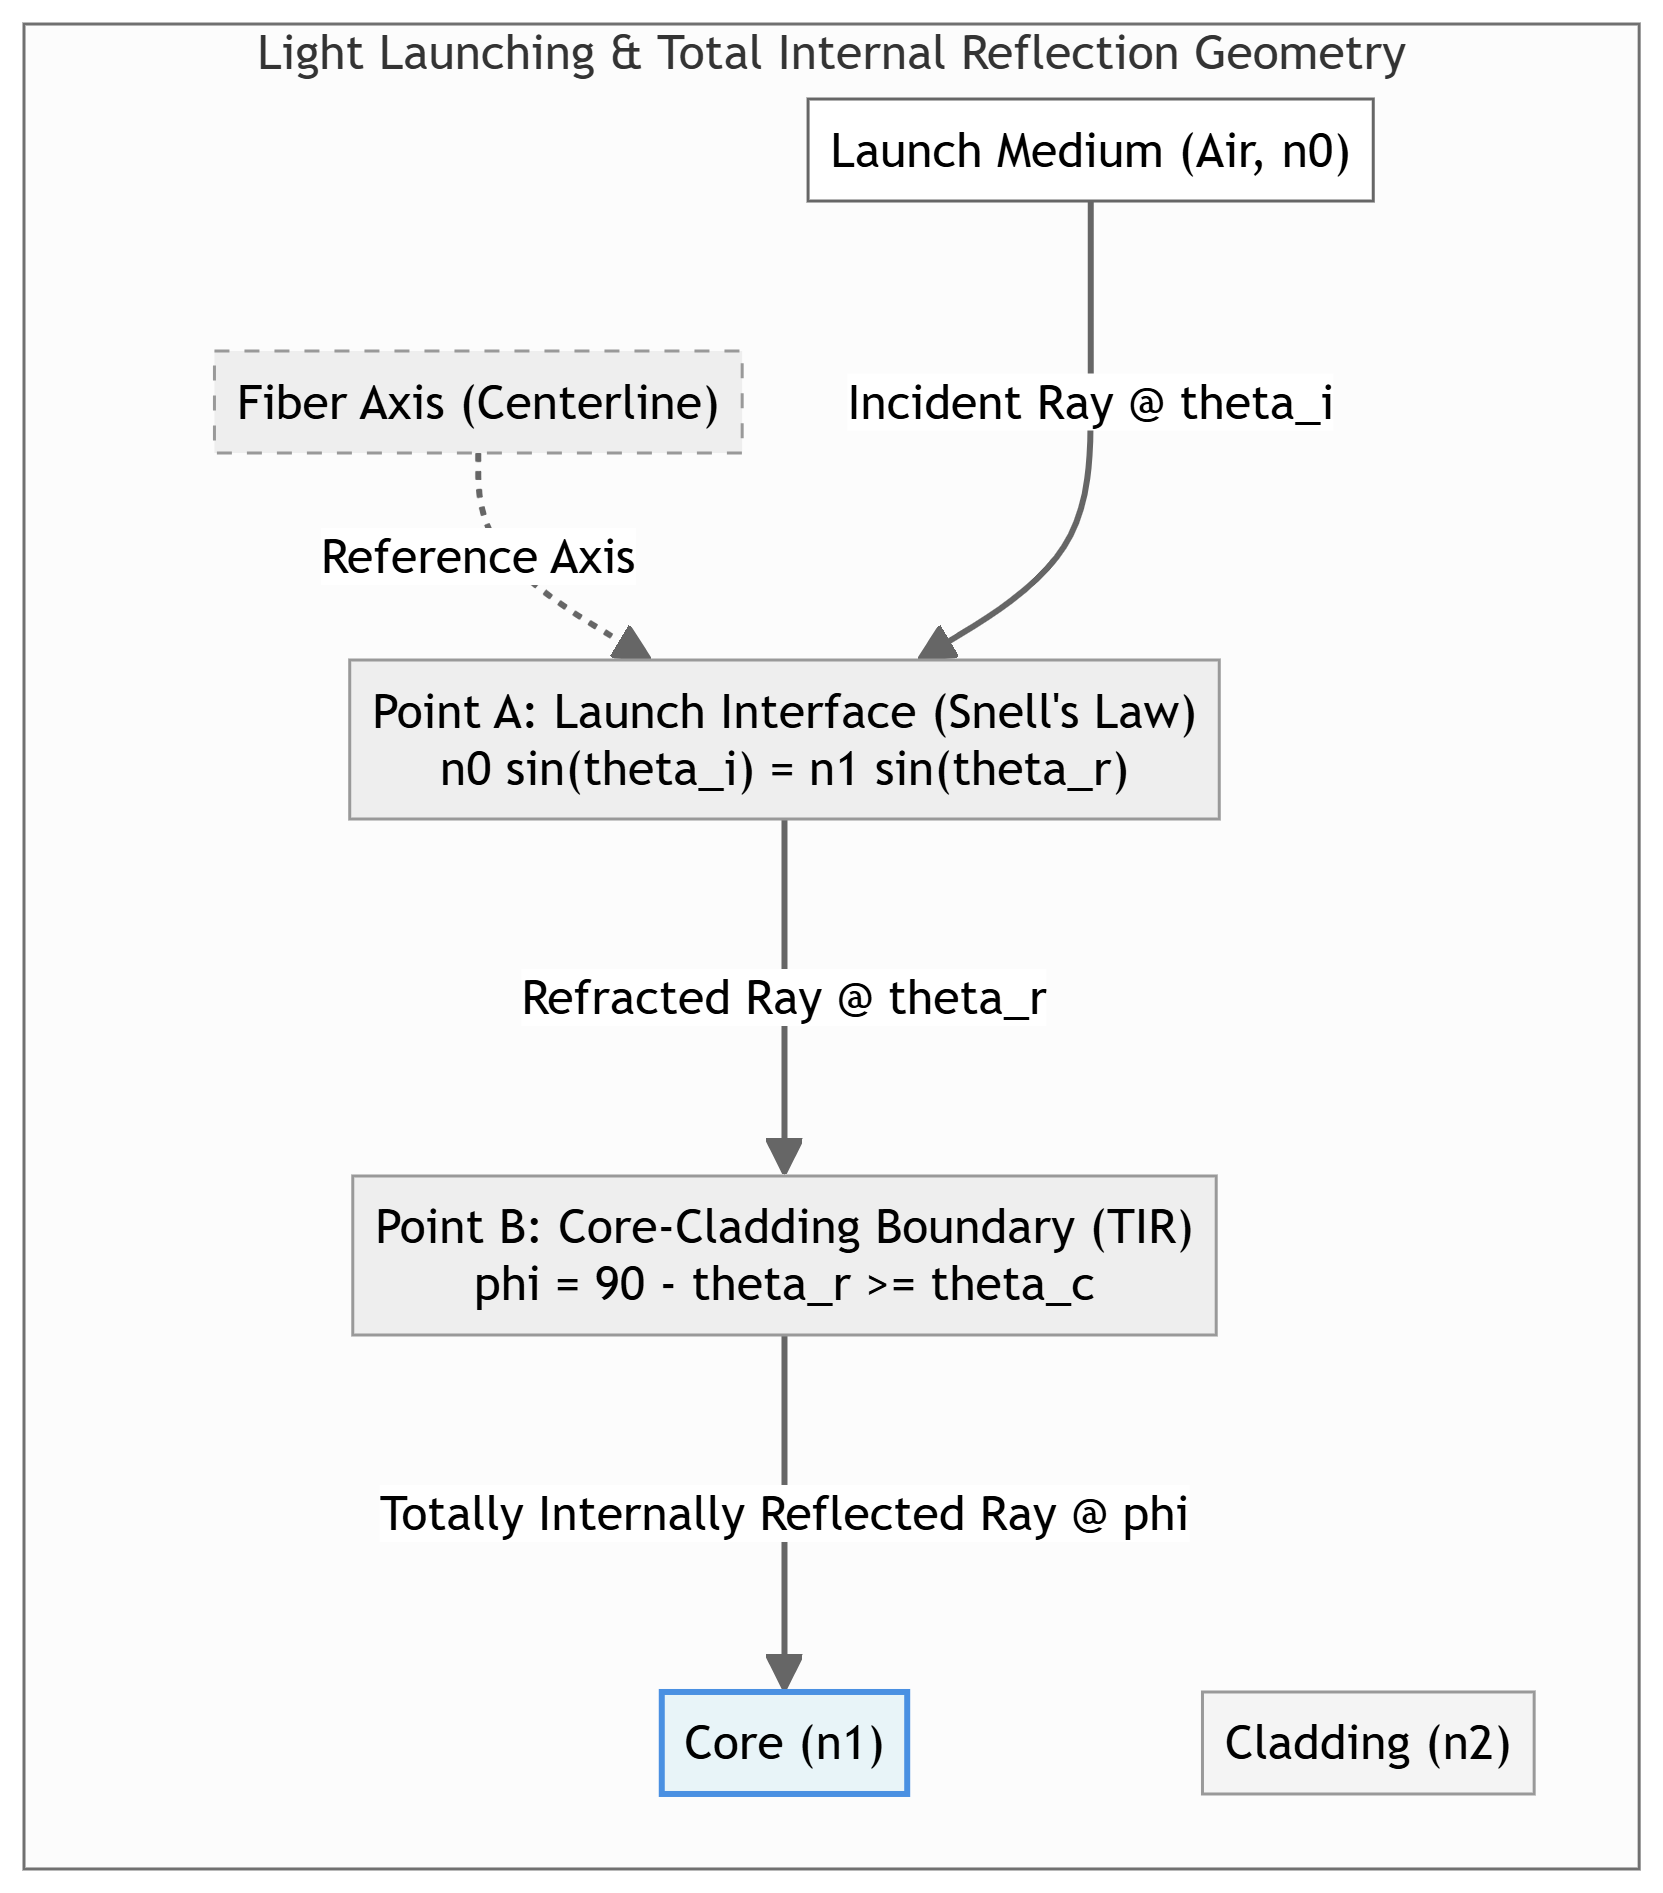
\includegraphics[width=0.75\textwidth,height=0.32\textheight,keepaspectratio]{../Images/chapter_01/ray_propagation.png}
\caption{Ray Propagation \& Angles}
\end{figure}

\subsection{3. Attenuation Curve \& Transmission Windows (Unit III)}
Wavelength dependent attenuation showing Rayleigh scattering, infrared absorption, and the $1310/1550\text{ nm}$ windows.  
\begin{figure}[H]
\centering
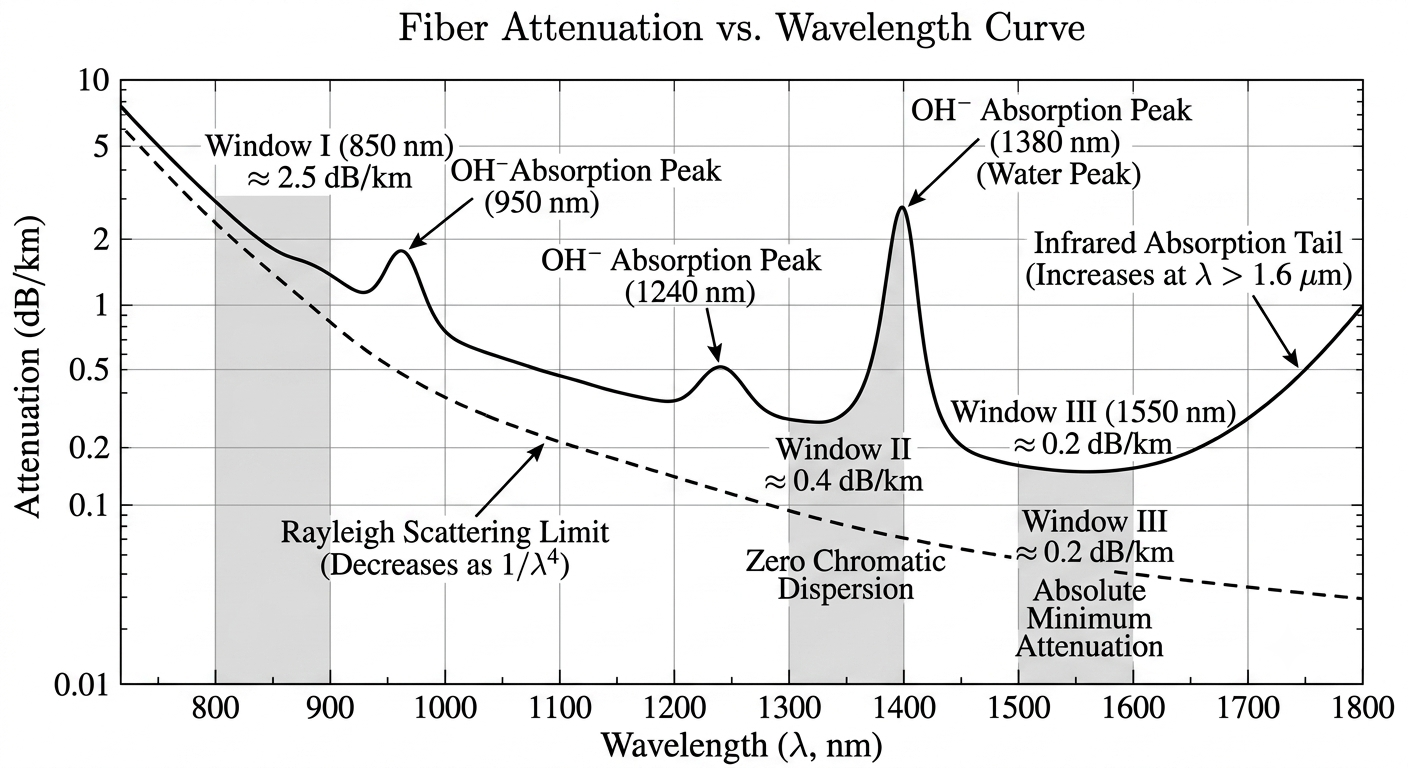
\includegraphics[width=0.75\textwidth,height=0.32\textheight,keepaspectratio]{../Images/chapter_03/attenuation_curve.png}
\caption{Attenuation Curve \& Transmission Windows}
\end{figure}

\subsection{4. Multimode vs. Single-Mode Pulse Broadening (Unit III)}
Illustration of how multiple paths lead to dispersion and overlapping output pulses.  
\begin{figure}[H]
\centering
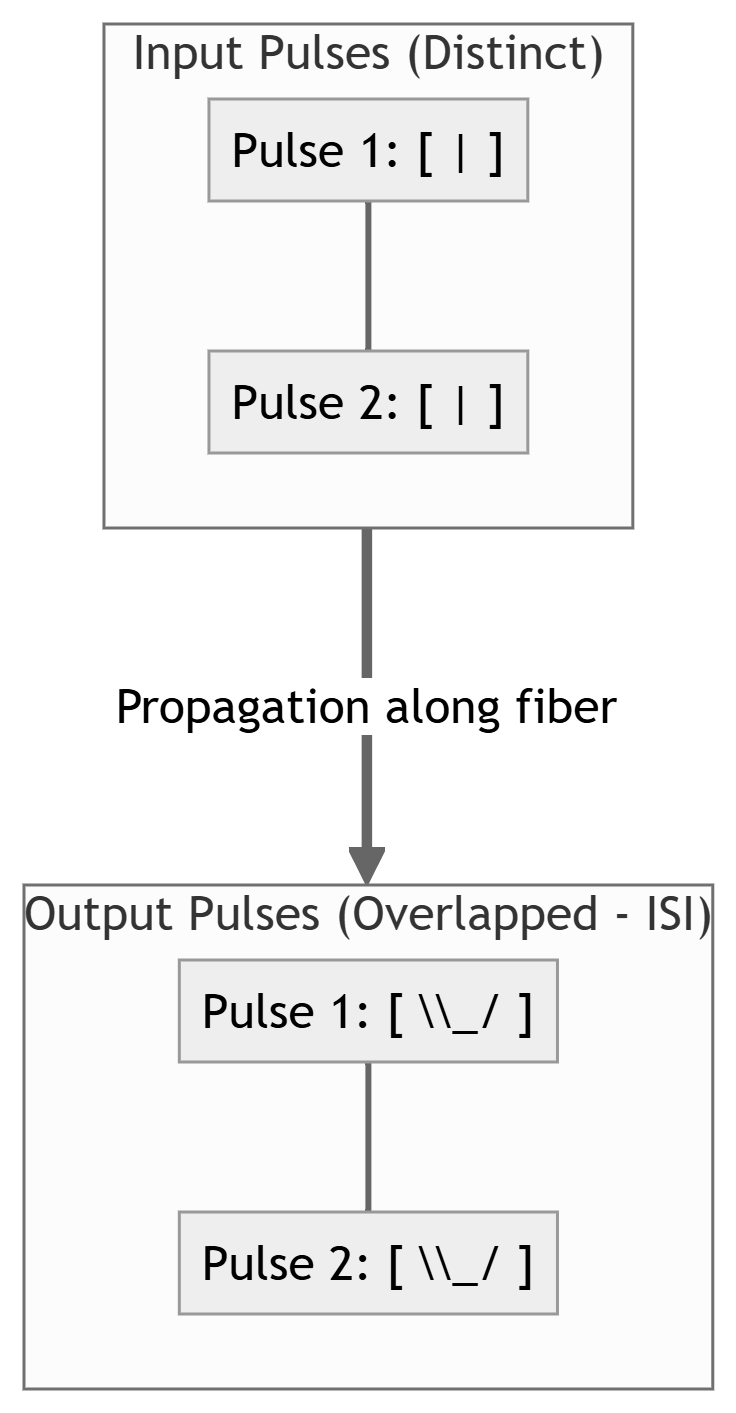
\includegraphics[width=0.75\textwidth,height=0.32\textheight,keepaspectratio]{../Images/chapter_03/pulse_broadening.png}
\caption{Pulse Broadening}
\end{figure}

\subsection{5. OTDR Configuration \& Trace (Unit III)}
OTDR optical splitter block diagram and the corresponding backscatter log trace identifying splices, faults, and reflection peaks.  
\begin{figure}[H]
\centering
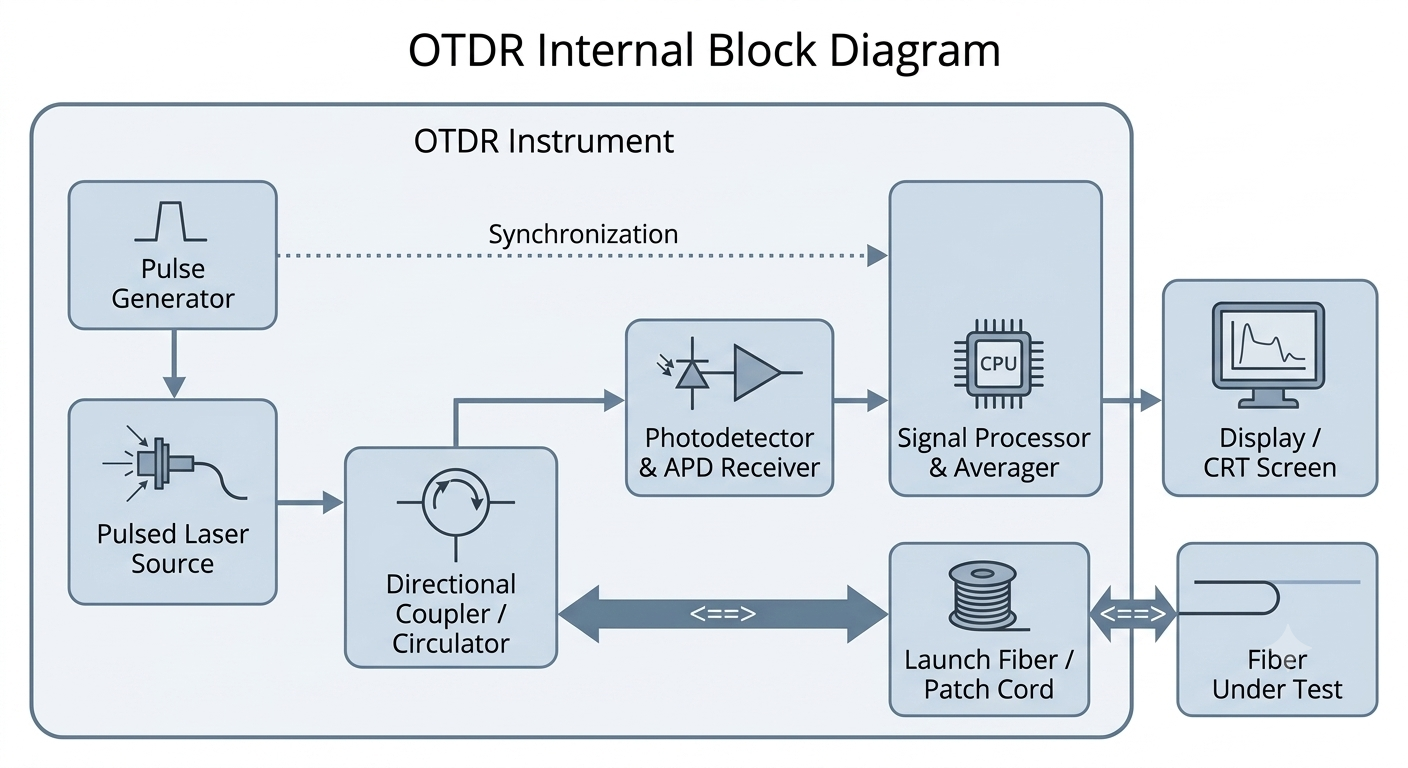
\includegraphics[width=0.75\textwidth,height=0.32\textheight,keepaspectratio]{../Images/chapter_03/otdr_block.png}
\caption{OTDR block diagram}
\end{figure}
\begin{figure}[H]
\centering
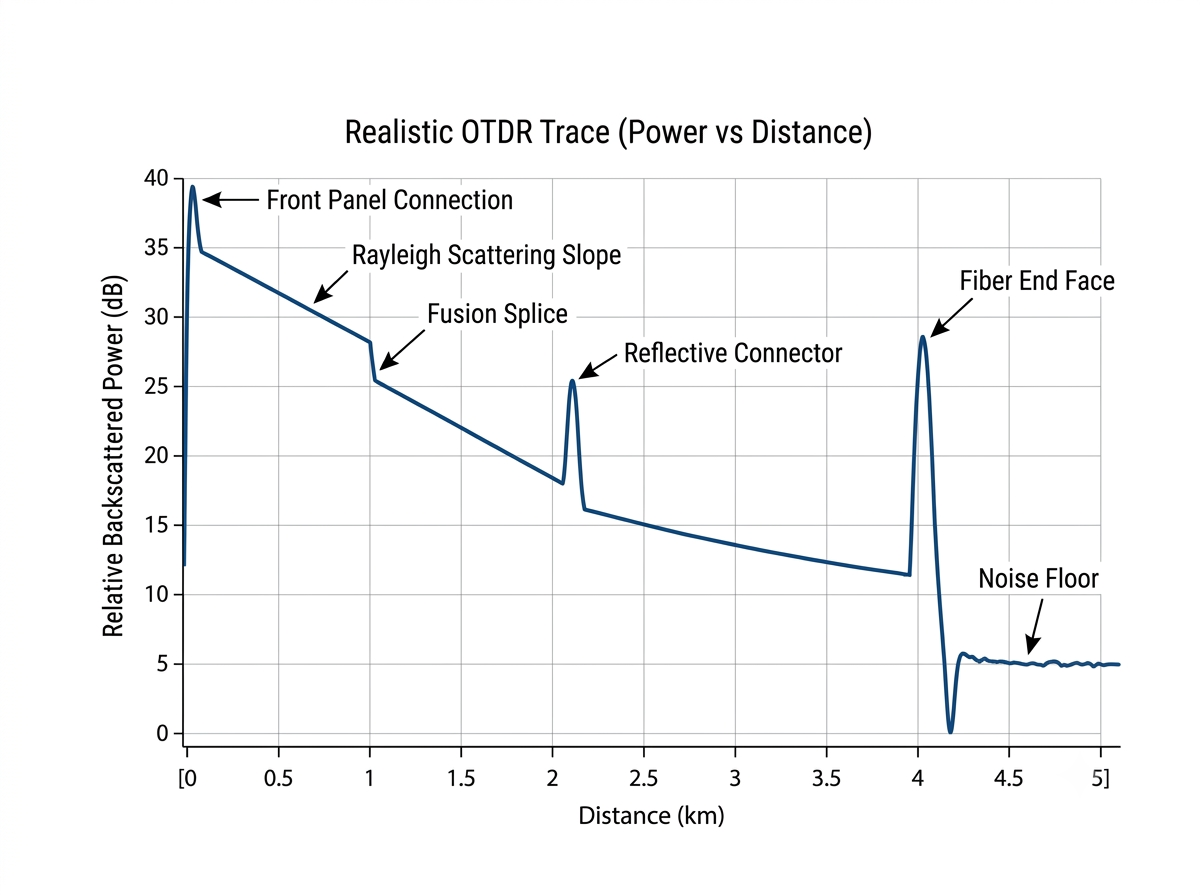
\includegraphics[width=0.75\textwidth,height=0.32\textheight,keepaspectratio]{../Images/chapter_03/otdr_trace.png}
\caption{OTDR trace}
\end{figure}

\subsection{6. Laser Resonator Cavity (Unit IV)}
Double-heterostructure gain medium with cleaved mirror end-facets highlighting optical feedback.  
\begin{figure}[H]
\centering
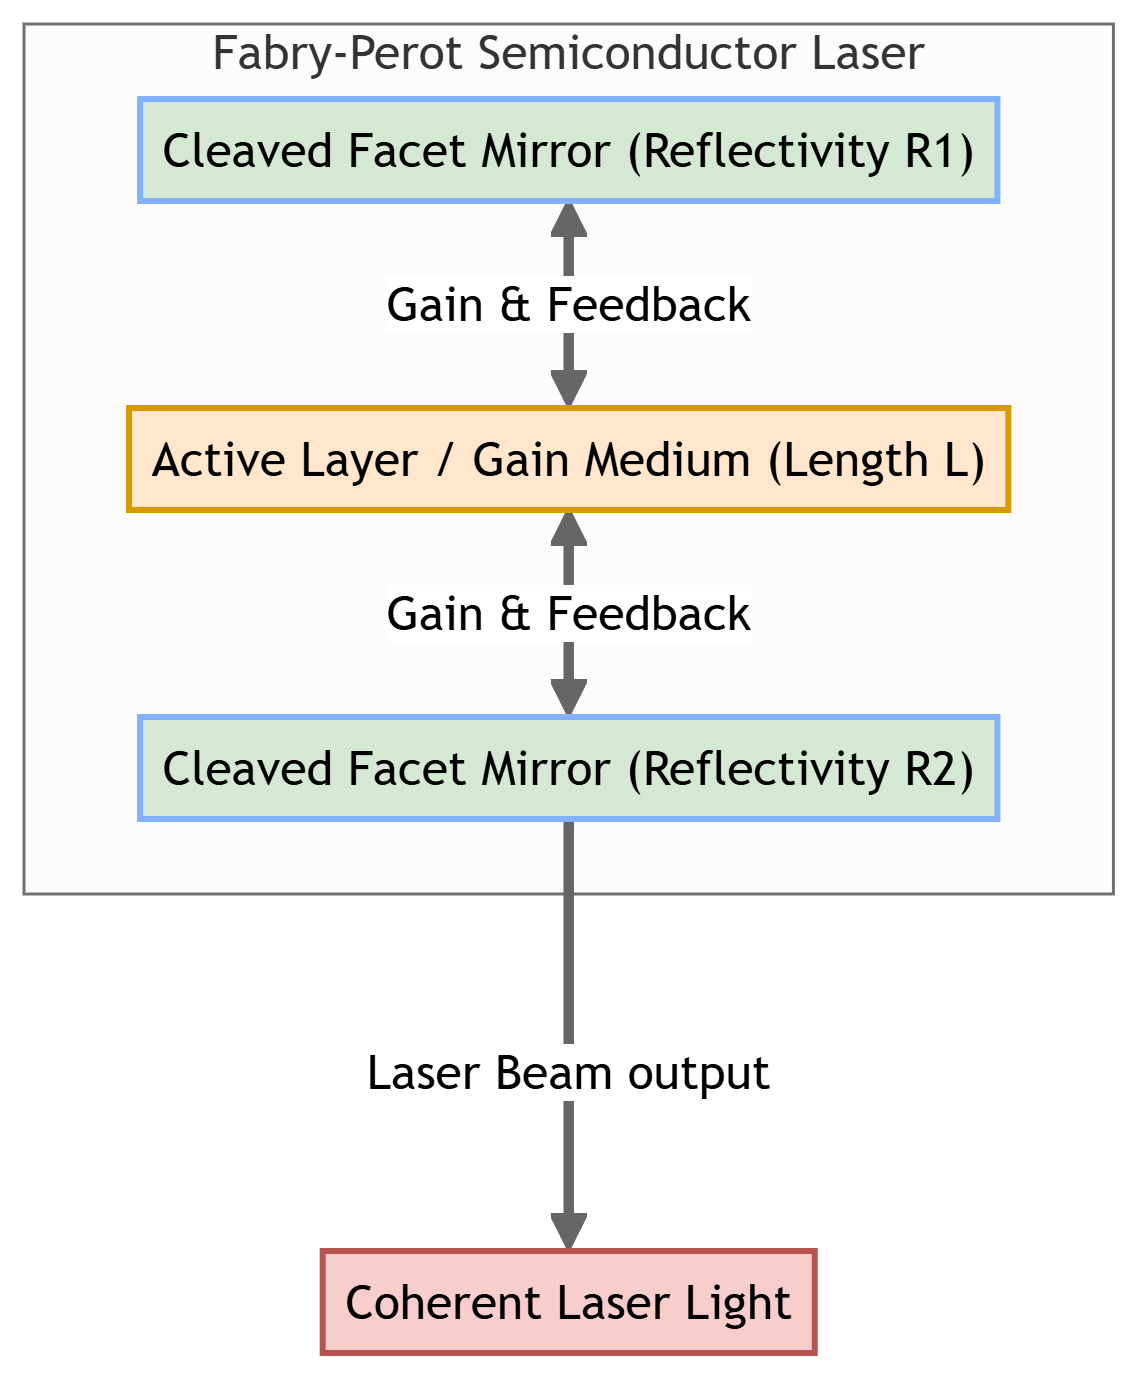
\includegraphics[width=0.75\textwidth,height=0.32\textheight,keepaspectratio]{../Images/chapter_04/laser_cavity.png}
\caption{Laser Cavity structure}
\end{figure}

\subsection{7. Digital Optical Receiver Pipeline (Unit IV)}
Block diagram tracking signal from photodiode through pre-amplifier, filter, and decision circuit.  
\begin{figure}[H]
\centering
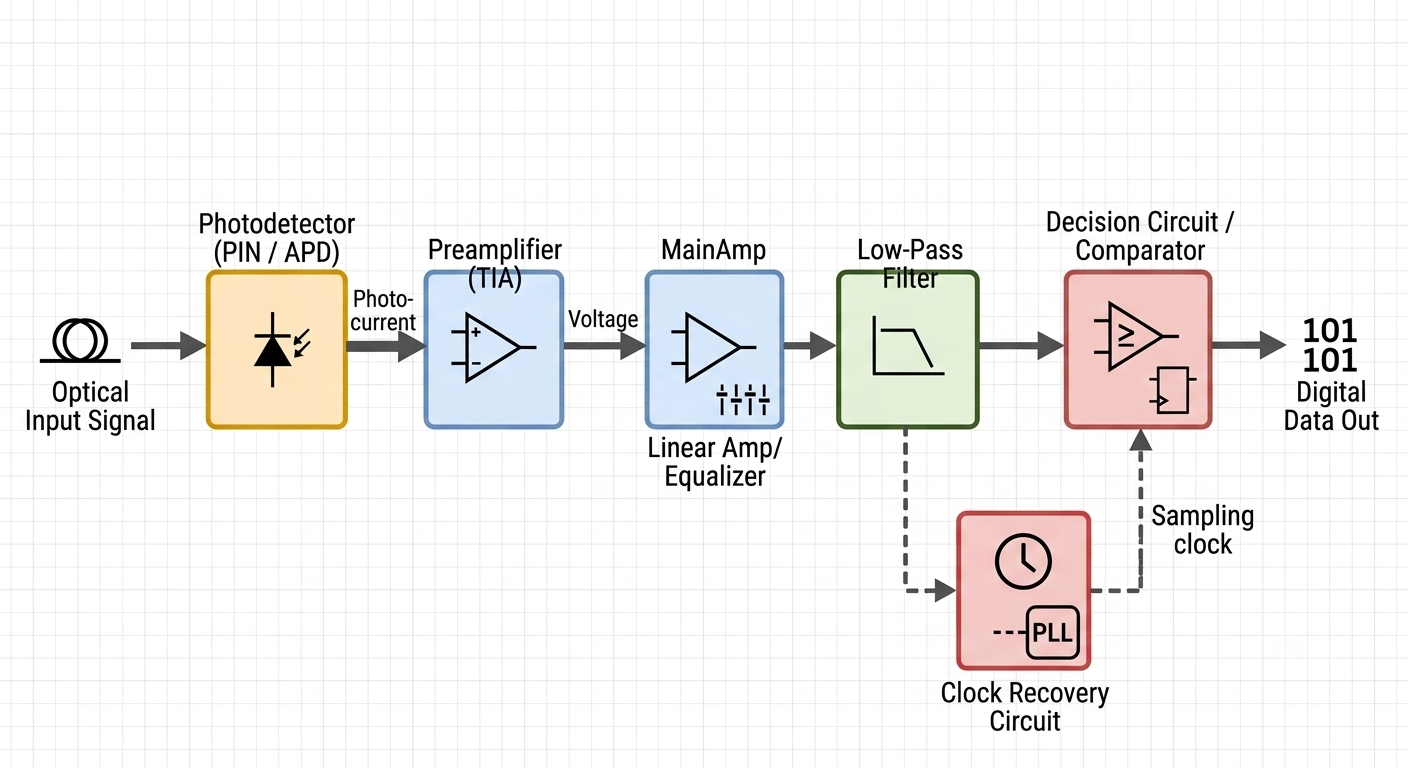
\includegraphics[width=0.75\textwidth,height=0.32\textheight,keepaspectratio]{../Images/chapter_04/optical_receiver.png}
\caption{Optical Receiver structure}
\end{figure}

\subsection{8. EDFA Physical Layout (Unit V)}
Optical configuration detailing Erbium spool, pump laser, WDM coupler, and input/output isolators.  
\begin{figure}[H]
\centering
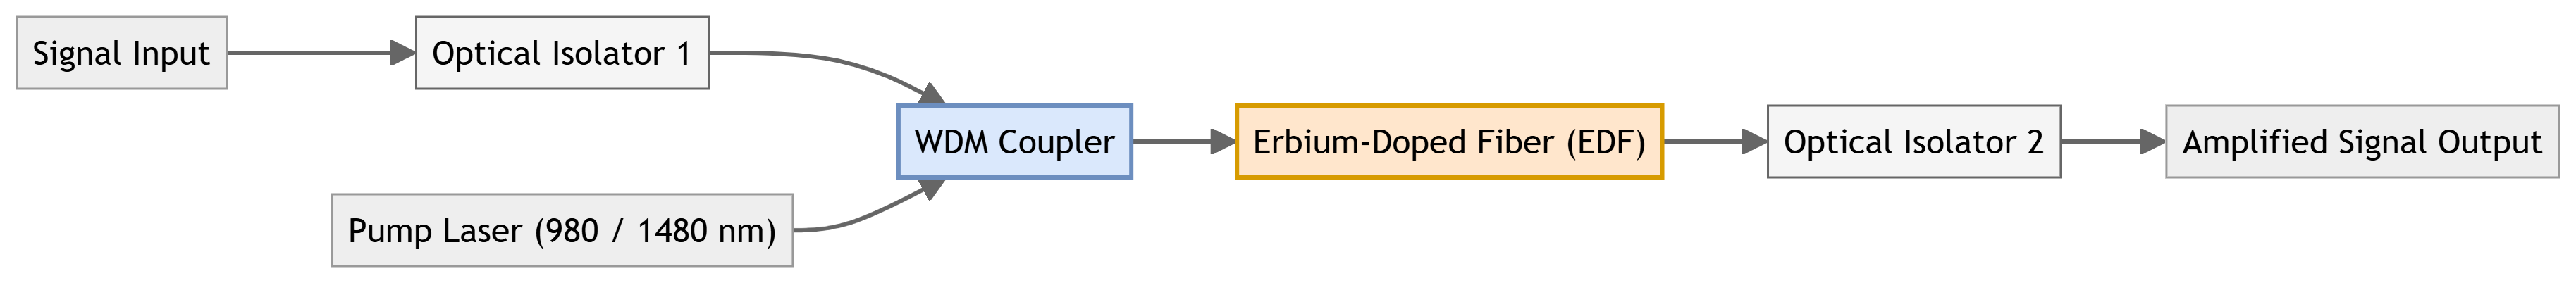
\includegraphics[width=0.75\textwidth,height=0.32\textheight,keepaspectratio]{../Images/chapter_05/edfa_block.png}
\caption{EDFA Block diagram}
\end{figure}

\subsection{9. Directional Coupler States (Unit V)}
Layout showing coupling paths for Cross State (zero volts) and Bar State (voltage applied).  
\begin{figure}[H]
\centering
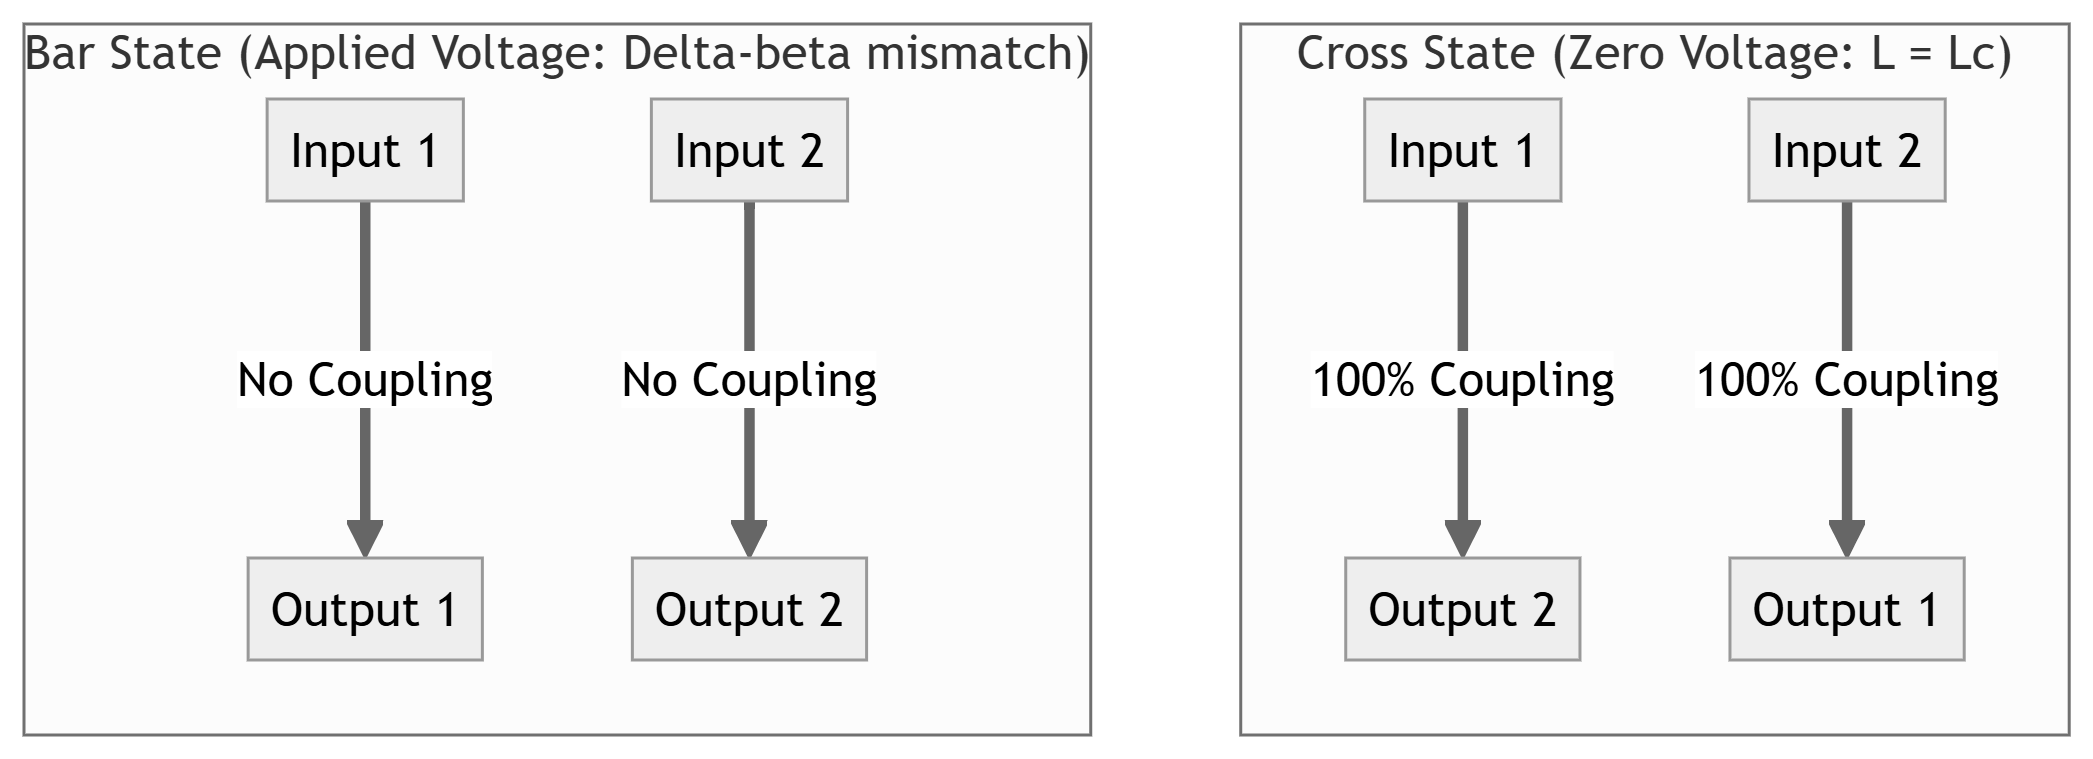
\includegraphics[width=0.75\textwidth,height=0.32\textheight,keepaspectratio]{../Images/chapter_05/directional_coupler.png}
\caption{Directional Coupler Switch States}
\end{figure}

\subsection{10. MZI Optical Switch Layout (Unit V)}
Y-splitter arms with deposited metal electrodes creating phase difference via electro-optic index shift.  
\begin{figure}[H]
\centering
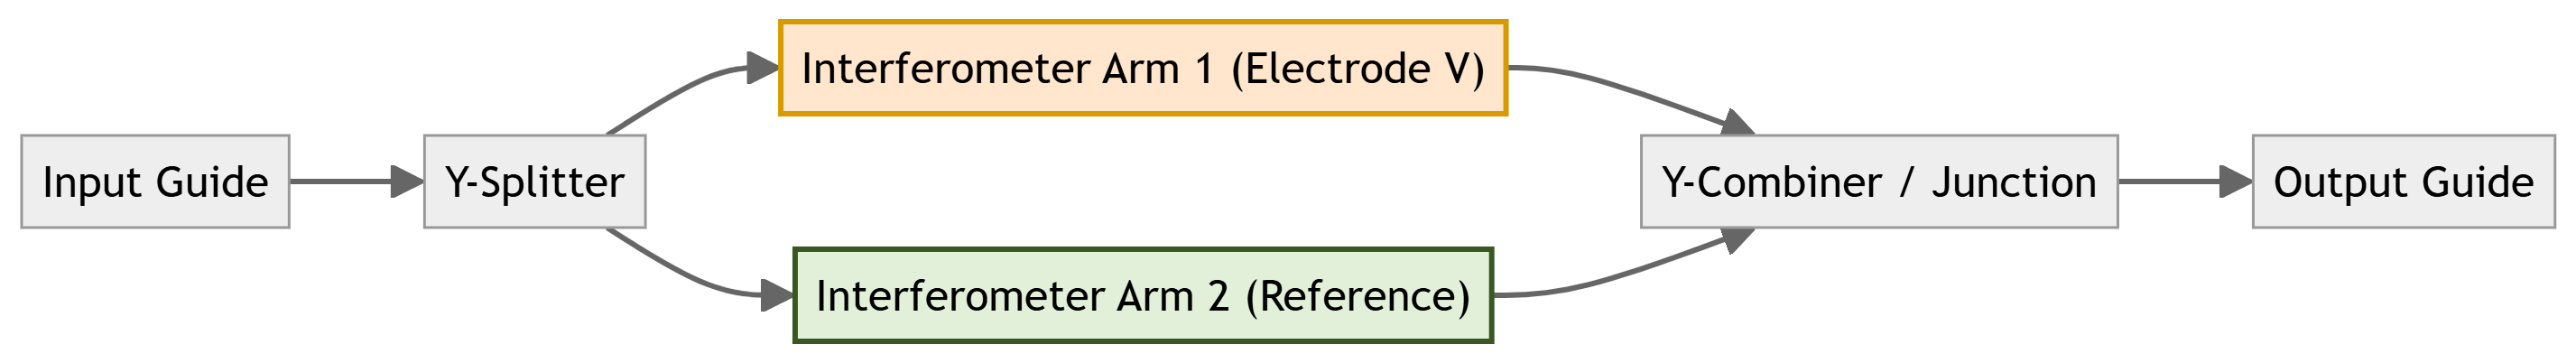
\includegraphics[width=0.75\textwidth,height=0.32\textheight,keepaspectratio]{../Images/chapter_05/mzi_switch.png}
\caption{MZI Switch Layout}
\end{figure}

\subsection{11. OADM and OXC Routing Architectures (Unit V)}
Wavelength drop/add filters and cross-connect fiber routing tables.  
\begin{figure}[H]
\centering
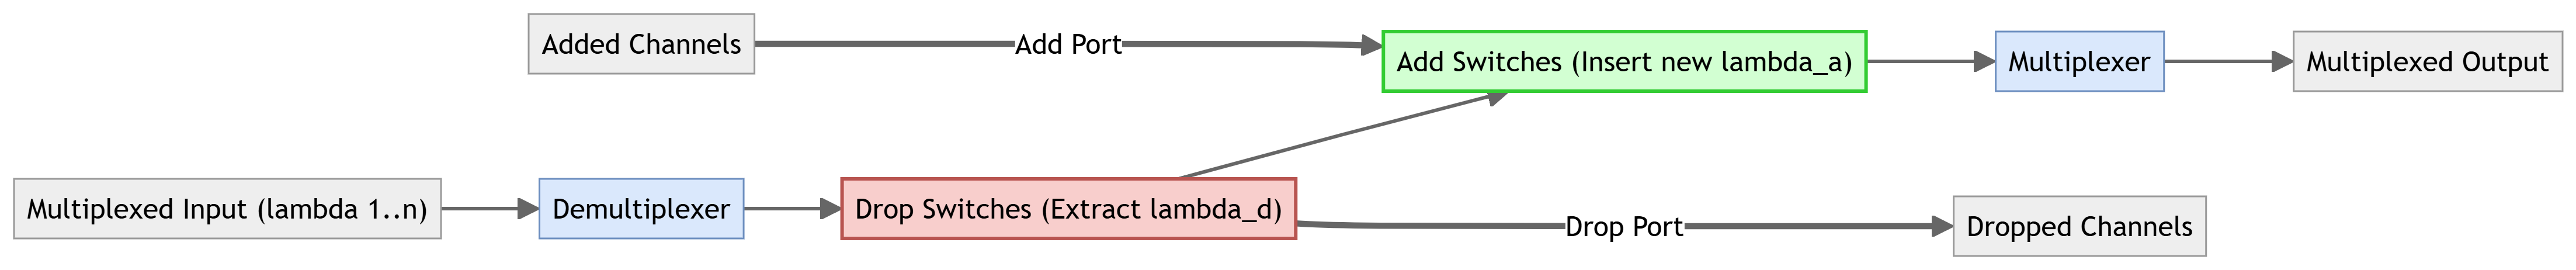
\includegraphics[width=0.75\textwidth,height=0.32\textheight,keepaspectratio]{../Images/chapter_05/oadm_block.png}
\caption{OADM Architecture}
\end{figure}
\begin{figure}[H]
\centering
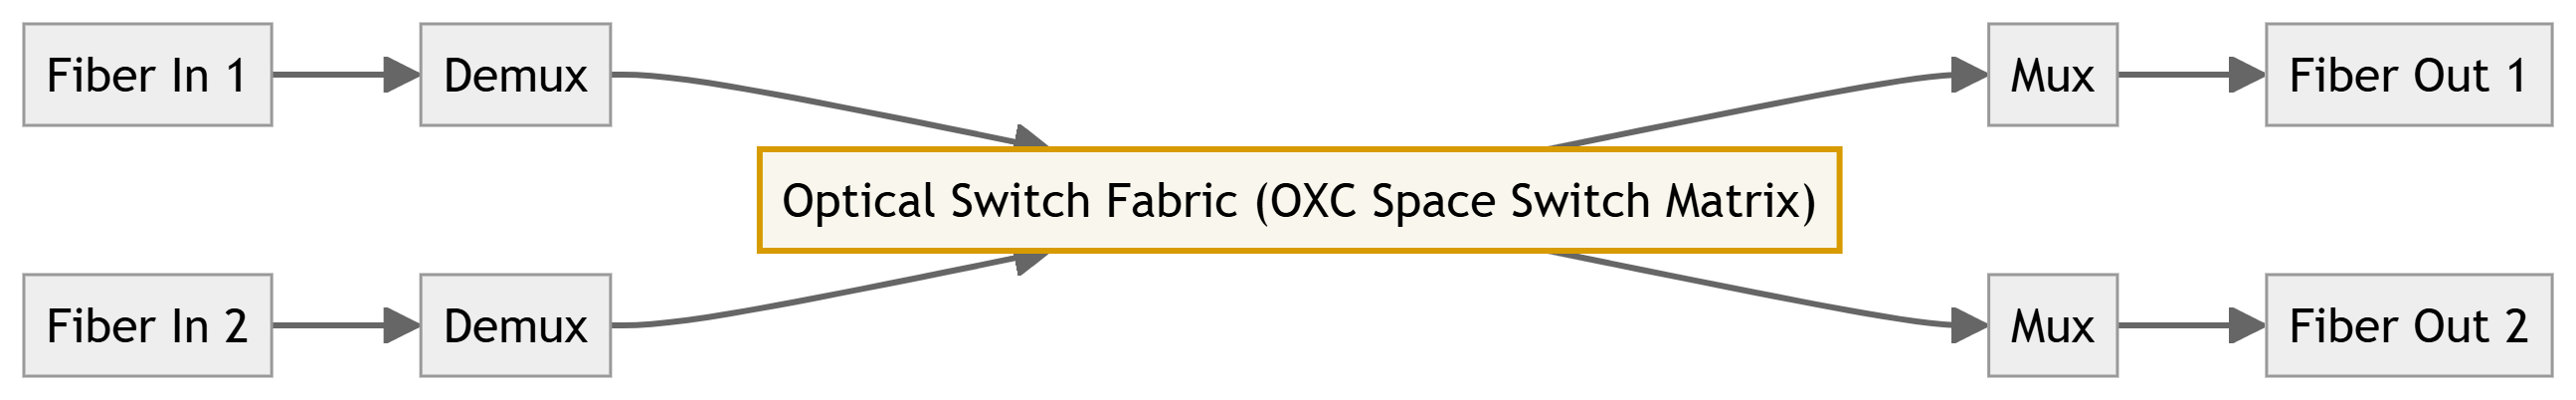
\includegraphics[width=0.75\textwidth,height=0.32\textheight,keepaspectratio]{../Images/chapter_05/oxc_routing.png}
\caption{OXC Wavelength Routing}
\end{figure}

\subsection{12. SRS vs. SBS Scattering Processes (Unit VI)}
Energy transition flowcharts comparing optical molecular phonons (SRS) vs. acoustic density wave phonons (SBS).  
\begin{figure}[H]
\centering
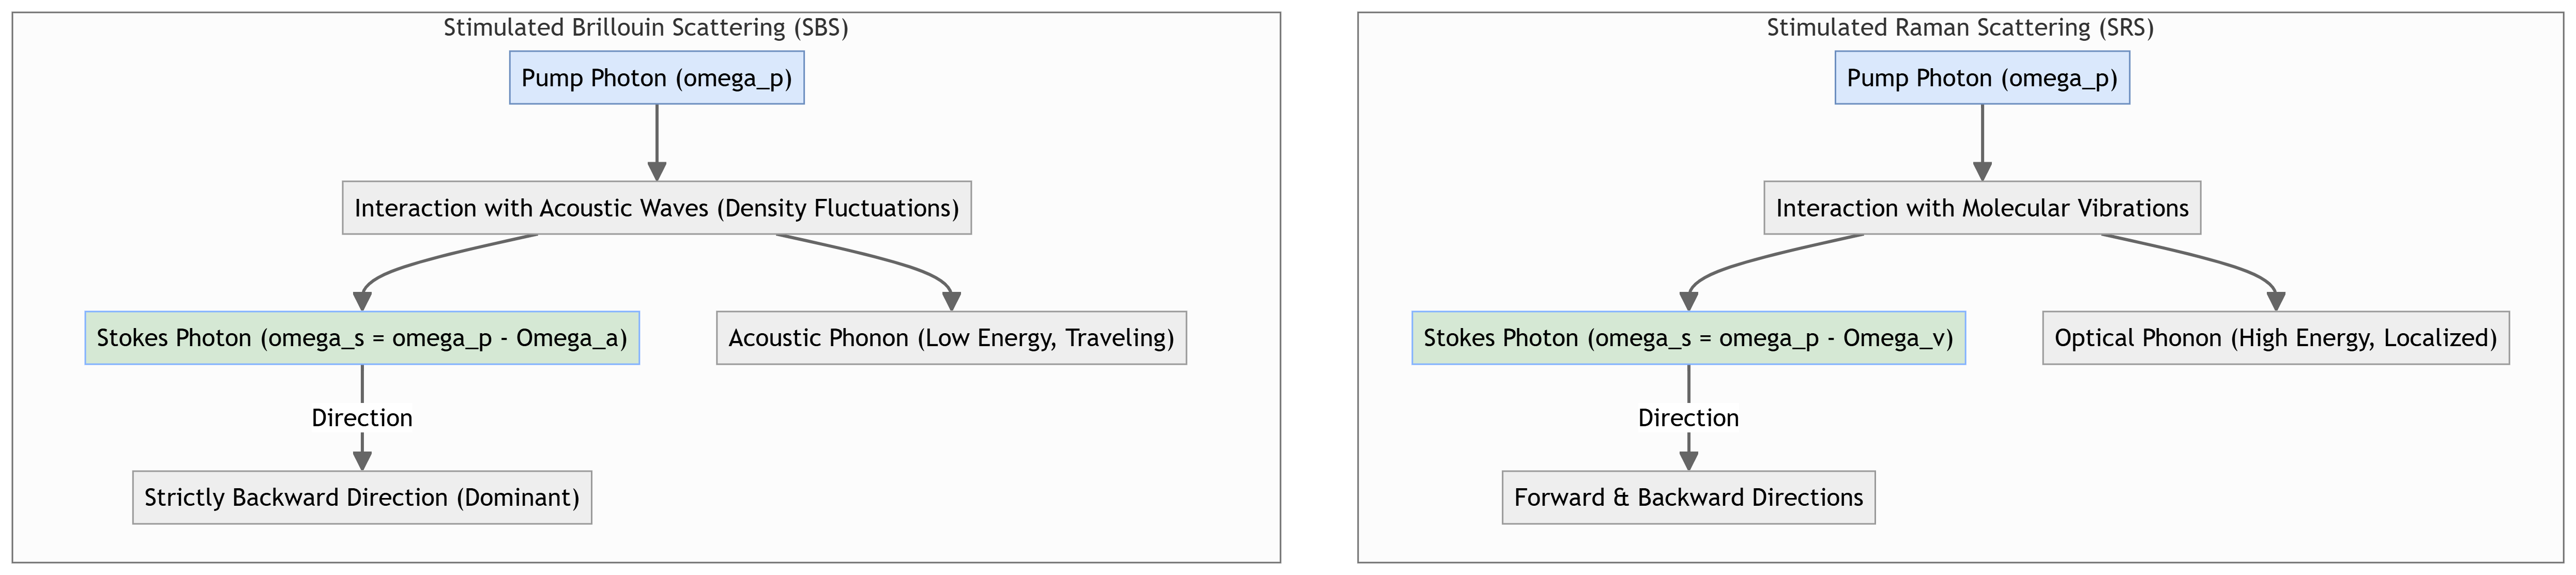
\includegraphics[width=0.75\textwidth,height=0.32\textheight,keepaspectratio]{../Images/chapter_06/srs_vs_sbs.png}
\caption{SRS vs. SBS scattering}
\end{figure}

\subsection{13. SPM Pulse Chirping (Unit VI)}
Envelope index changes mapping leading edge red shifts and trailing edge blue shifts.  
\begin{figure}[H]
\centering
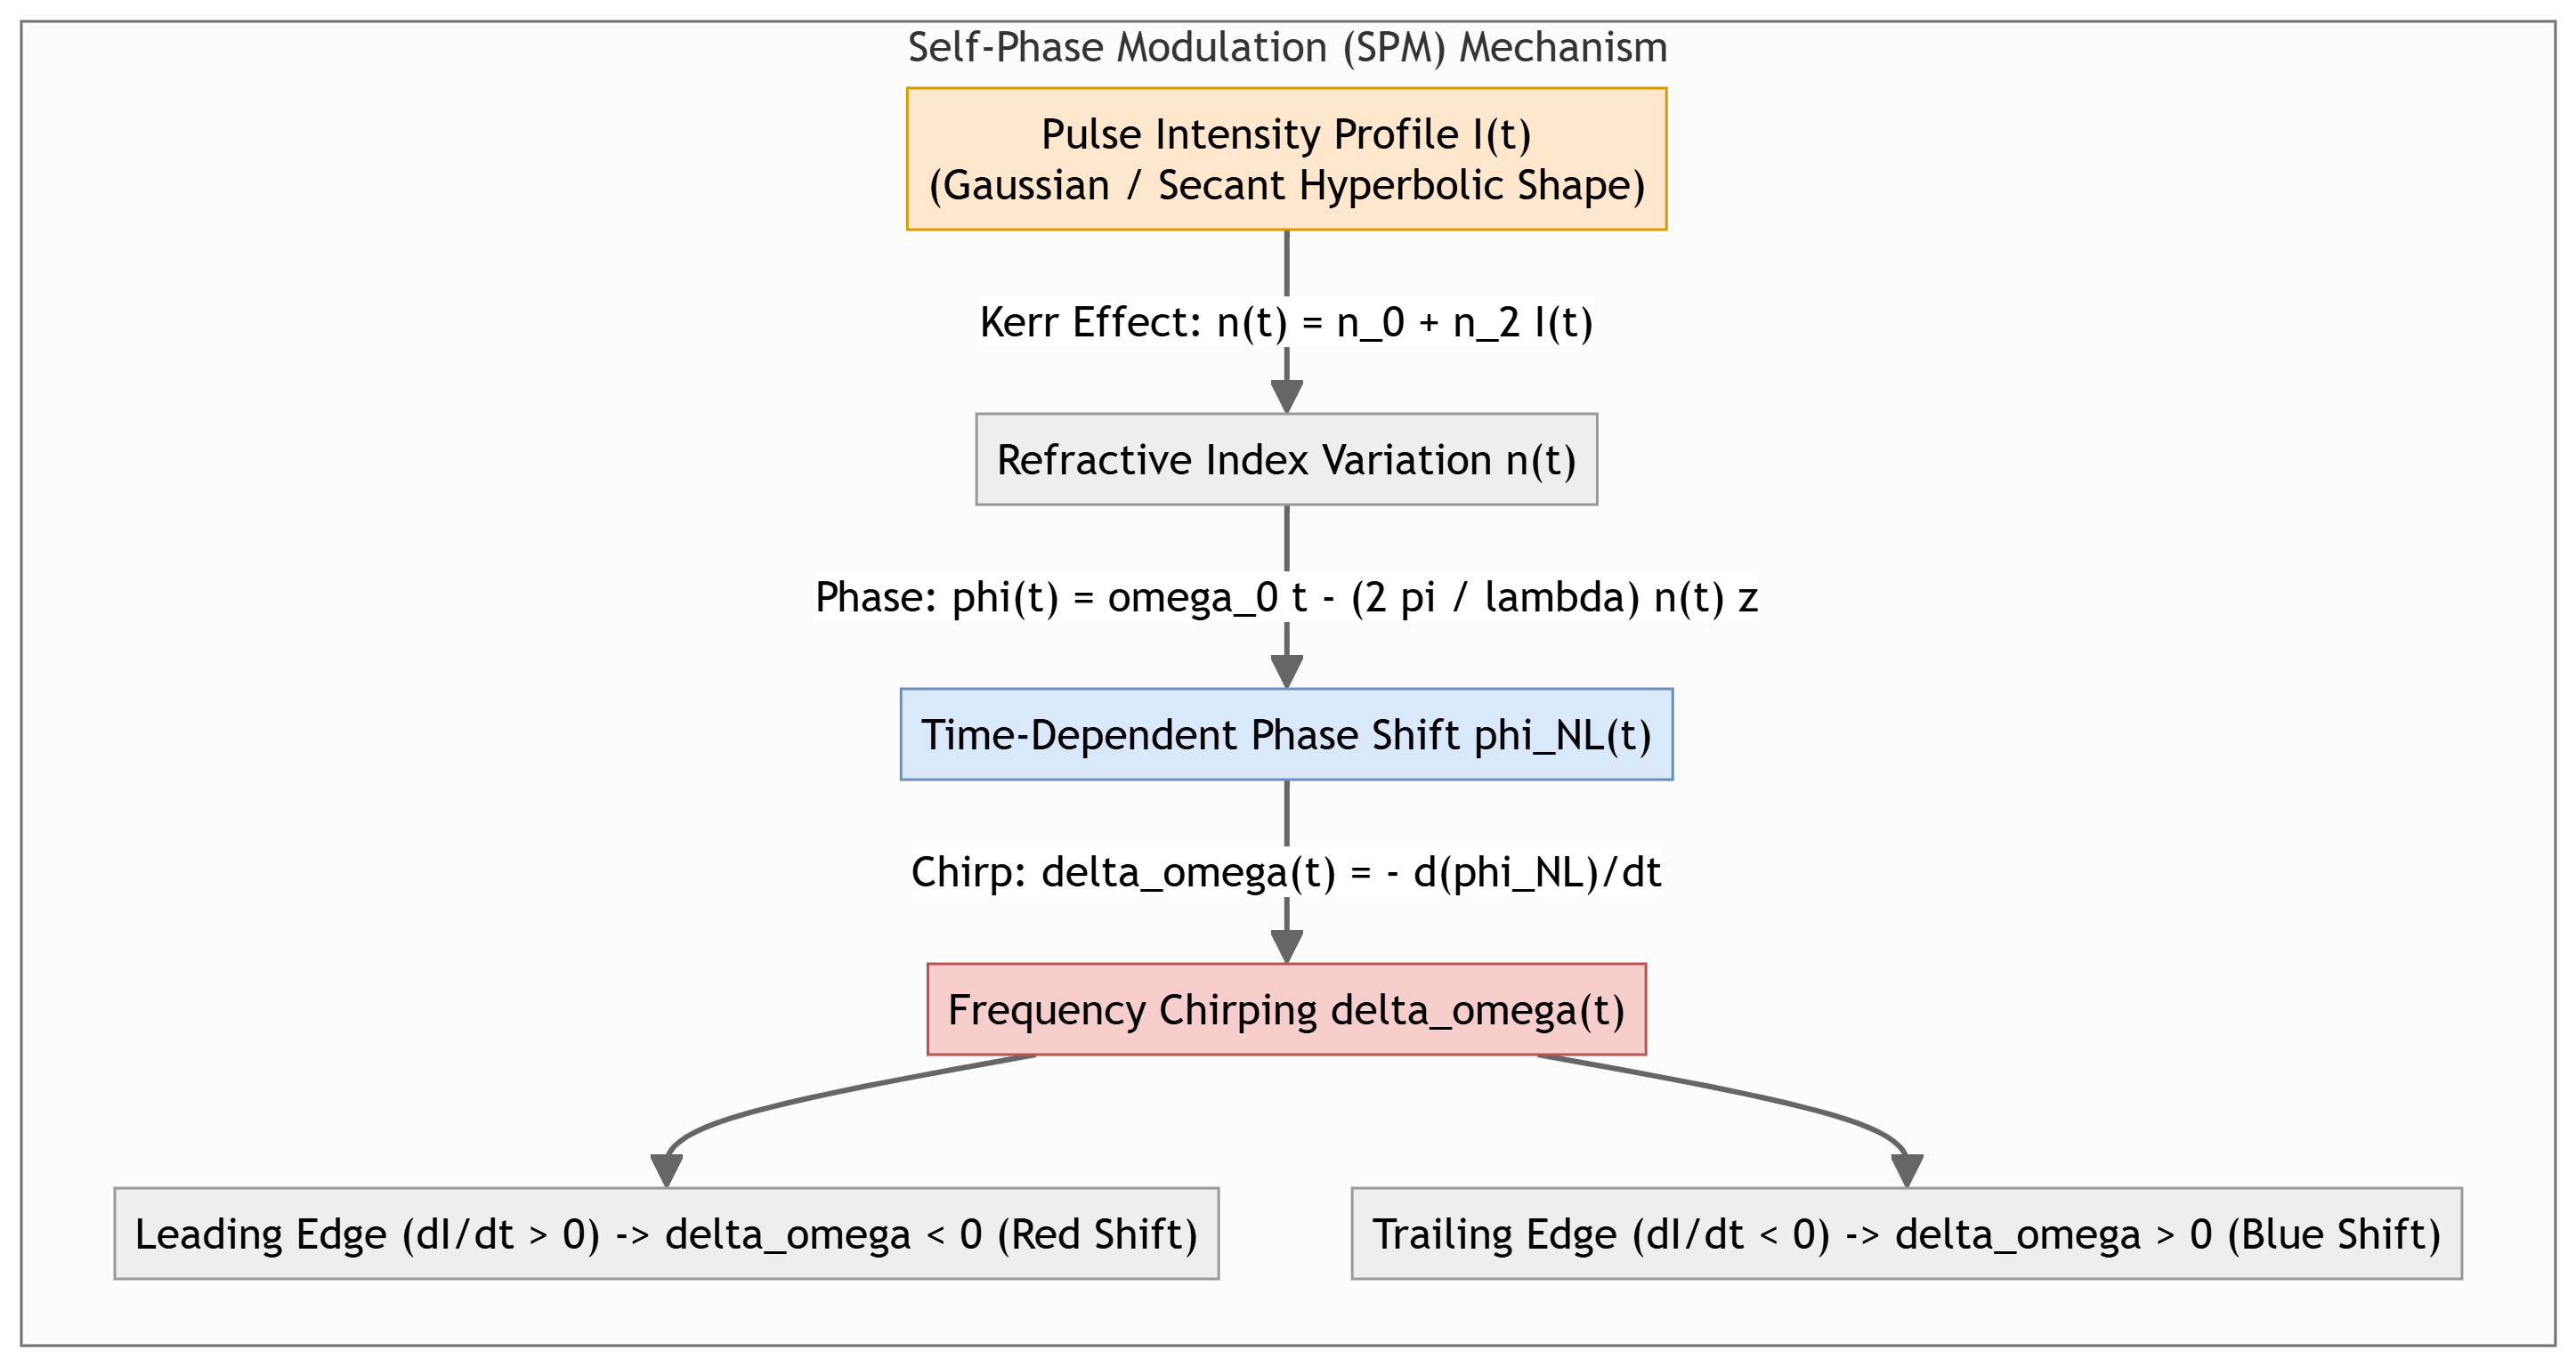
\includegraphics[width=0.75\textwidth,height=0.32\textheight,keepaspectratio]{../Images/chapter_06/spm_chirp.png}
\caption{SPM frequency chirping}
\end{figure}

\subsection{14. Soliton Envelope Balance (Unit VI)}
Interaction curve showing anomalous GVD compression exactly counteracting SPM broadening.  
\begin{figure}[H]
\centering
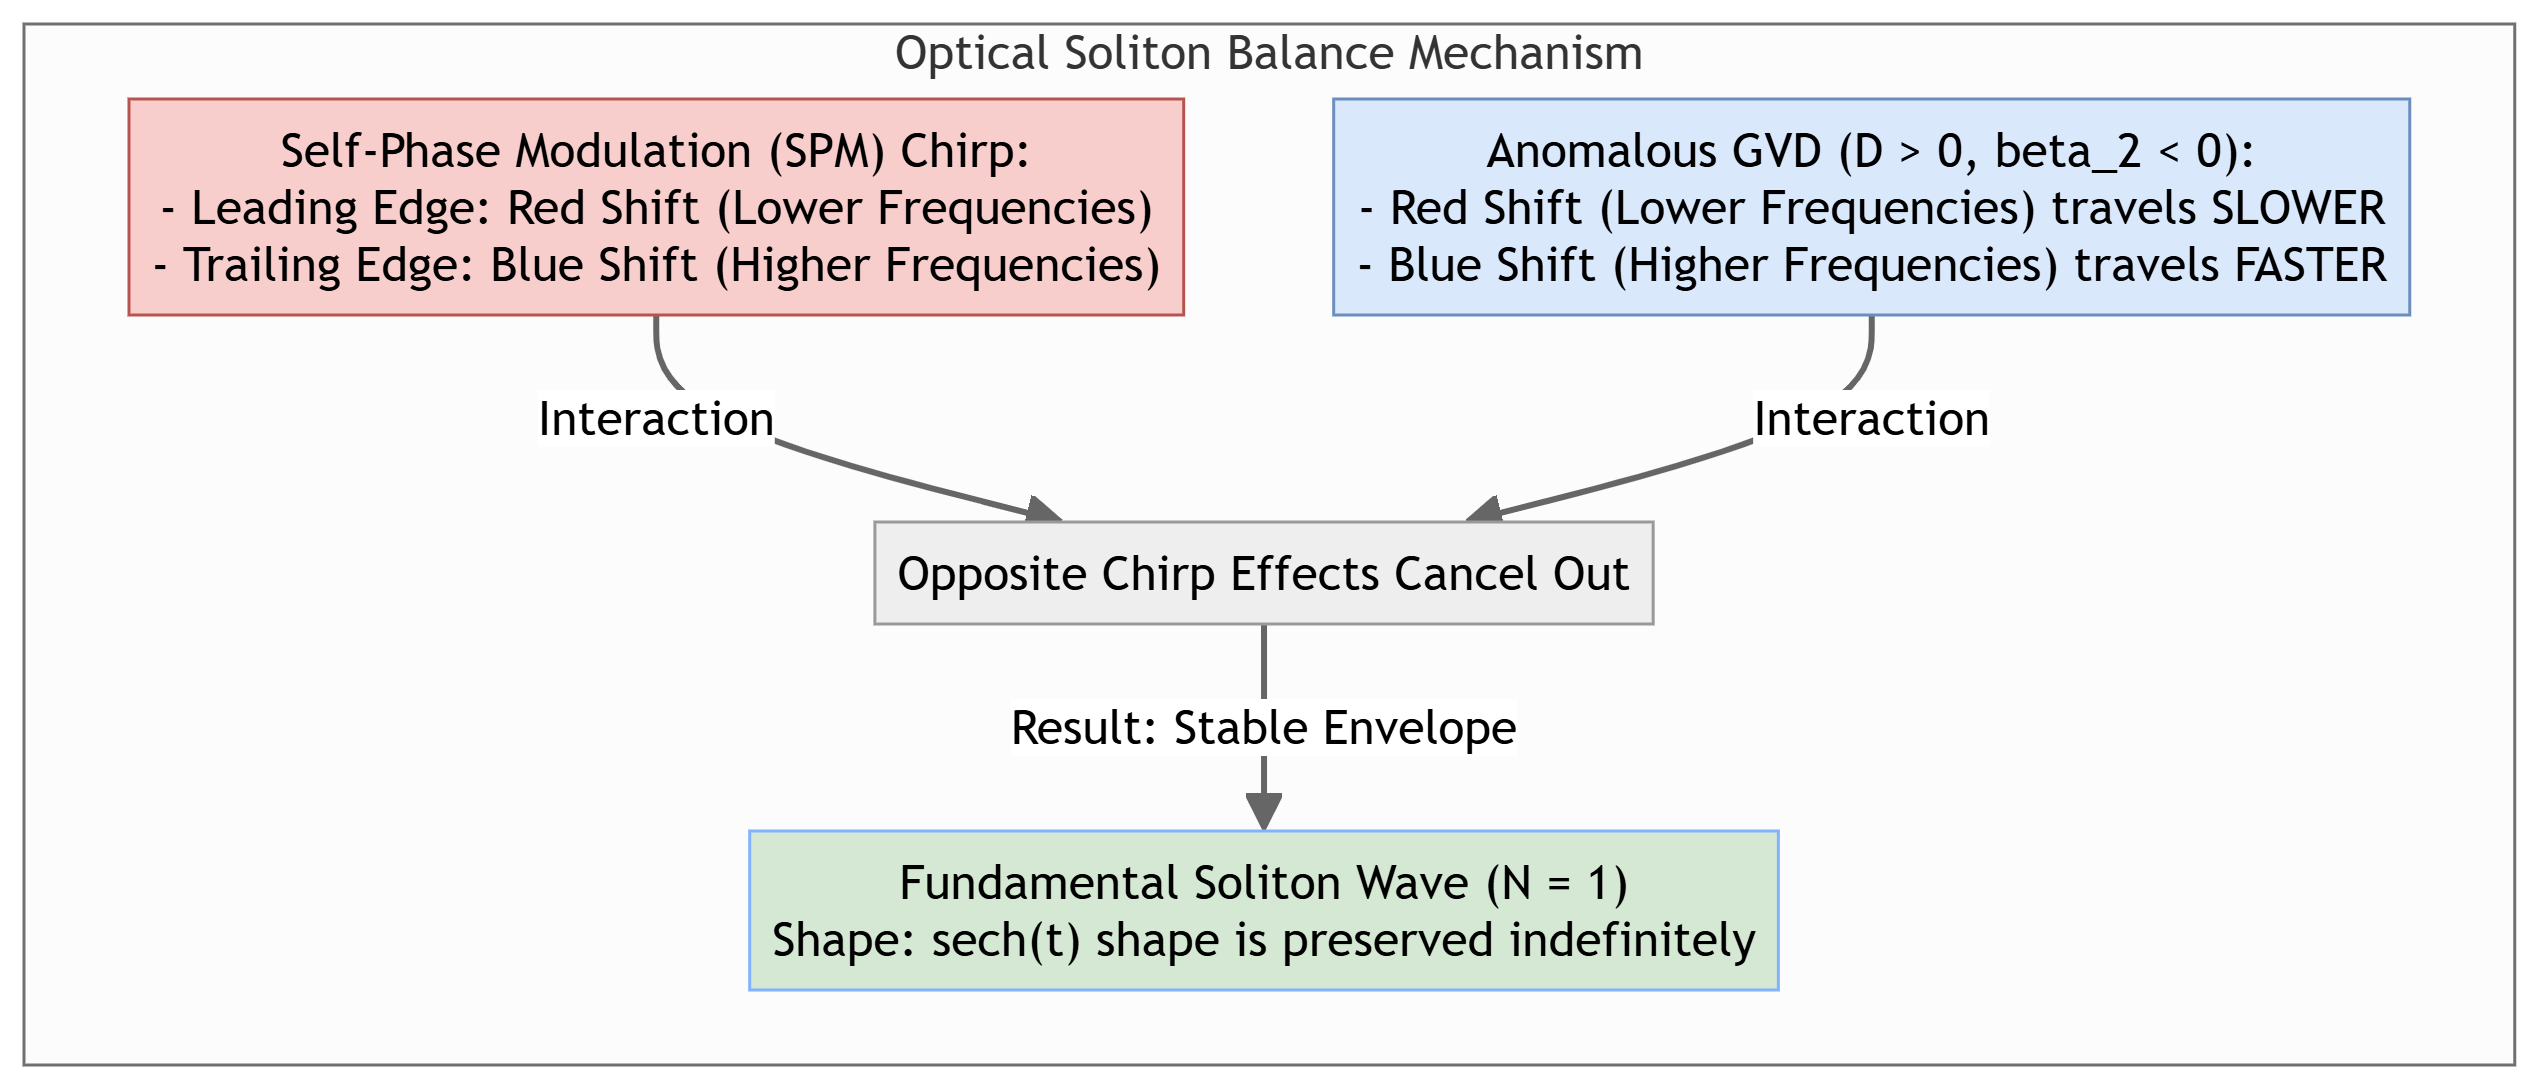
\includegraphics[width=0.75\textwidth,height=0.32\textheight,keepaspectratio]{../Images/chapter_06/soliton_balance.png}
\caption{Soliton propagation balance}
\end{figure}


\section{Frequently Asked Questions}

\subsection{Q1. Derive the expression for Acceptance Angle and Numerical Aperture (NA) of a multimode step-index fiber. [10M]}
\begin{itemize}
  \item   \textbf{Step 1:} Consider a ray of light entering the fiber core from a medium of refractive index $n_0$ (air, $n_0 = 1$) at an angle $\theta_0$ to the fiber axis.
  \item   \textbf{Step 2:} Apply Snell's Law at the air-core interface:
\end{itemize}
    \[ n_0 \sin \theta_0 = n_1 \sin \theta_1 \]
\begin{itemize}
  \item   \textbf{Step 3:} The refracted ray strikes the core-cladding boundary at an angle of incidence $\phi$. For total internal reflection to occur, $\phi \ge \theta_c$. From geometry:
\end{itemize}
    \[ \theta_1 = 90^\circ - \phi \implies \sin \theta_1 = \cos \phi \]
\begin{itemize}
  \item   \textbf{Step 4:} Substitute this into Snell's Law:
\end{itemize}
    \[ n_0 \sin \theta_0 = n_1 \cos \phi = n_1 \sqrt{1 - \sin^2 \phi} \]
\begin{itemize}
  \item   \textbf{Step 5:} Under critical conditions, $\sin \phi = \sin \theta_c = n_2/n_1$. Substituting this yields:
\end{itemize}
    \[ n_0 \sin \theta_a = n_1 \sqrt{1 - \left(\frac{n_2}{n_1}\right)^2} = \sqrt{n_1^2 - n_2^2} \]
\begin{itemize}
  \item   \textbf{Step 6:} Setting $n_0 = 1$ for air, we get the final expression for NA:
\end{itemize}
    \[ \text{NA} = \sin \theta_a = \sqrt{n_1^2 - n_2^2} \]

\subsection{Q2. Compare step-index and graded-index fibers in terms of profiles, ray paths, and intermodal dispersion. [5M]}
\begin{itemize}
  \item   \textbf{Refractive Index Profile:} Step-index has a constant index $n_1$ in the core with a step decrease at the cladding. Graded-index has a parabolic index profile decreasing from the core axis outward.
  \item   \textbf{Ray Propagation Path:} Light travels in zig-zag straight lines in step-index cores. In graded-index cores, rays bend continuously in sinusoidal, helical paths.
  \item   \textbf{Intermodal Dispersion:} High in step-index fibers because rays traveling at larger angles take longer paths. Low in graded-index fibers because rays traveling on longer outer paths travel faster (where refractive index is lower), keeping arrival times synchronized.
\end{itemize}

\subsection{Q3. Derive the intermodal delay difference ($\Delta\tau$) in a step-index fiber. [10M]}
\begin{itemize}
  \item   \textbf{Fastest Ray:} Propagates along the central longitudinal axis of length $L$. Travel time is:
\end{itemize}
    \[ t_{\text{min}} = \frac{L}{v} = \frac{L n_1}{c} \]
\begin{itemize}
  \item   \textbf{Slowest Ray:} Travels at the critical angle $\theta_c$, reflecting repeatedly. Path length is $L/\sin \theta_c = L(n_1/n_2)$. Travel time is:
\end{itemize}
    \[ t_{\text{max}} = \frac{L (n_1/n_2)}{v} = \frac{L n_1^2}{c n_2} \]
\begin{itemize}
  \item   \textbf{Delay Difference ($\Delta\tau$):}
\end{itemize}
    \[ \Delta\tau = t_{\text{max}} - t_{\text{min}} = \frac{L n_1}{c} \left(\frac{n_1}{n_2} - 1\right) = \frac{L n_1}{c} \left(\frac{n_1 - n_2}{n_2}\right) \]
\begin{itemize}
  \item   Since $n_2 \approx n_1$ for weakly guiding fibers:
\end{itemize}
    \[ \Delta\tau \approx \frac{L n_1 \Delta}{c} \]

\subsection{Q4. Detail the differences between PIN photodiodes and Avalanche Photodiodes (APDs). [5M]}
\begin{itemize}
  \item   \textbf{Structure:} PIN photodiode has a standard Intrinsic semiconductor layer between P and N regions. APD has an additional high-field multiplication region.
  \item   \textbf{Gain Mechanism:} PIN photodiodes have no internal gain (one electron per photon, $M=1$). APDs provide internal gain ($M = 10 \text{ to } 100$) through avalanche multiplication.
  \item   \textbf{Responsivity:} PIN responsibility is lower ($\approx 0.6 \text{ to } 0.8\ \text{A/W}$). APD responsivity is much higher due to multiplication factor $M$.
  \item   \textbf{Noise \& Bias:} PIN photodiodes require low reverse bias voltage ($5 \text{ to } 15\ \text{V}$) and generate low noise. APDs require very high reverse bias voltage ($100 \text{ to } 300\ \text{V}$) and introduce excess avalanche noise.
\end{itemize}

\subsection{Q5. Differentiate between Erbium-Doped Fiber Amplifiers (EDFA) and Raman Amplifiers. [5M]}
\begin{itemize}
  \item   \textbf{Gain Medium:} EDFA uses a short, lumped section of silica fiber heavily doped with Erbium ions. Raman amplification uses the standard long transmission fiber itself (distributed gain).
  \item   \textbf{Amplification Principle:} EDFA uses stimulated emission from excited Erbium ions. Raman uses Stimulated Raman Scattering (SRS) where high-power pump photons transfer energy to signal photons.
  \item   \textbf{Operating Band:} EDFA is restricted to the fixed C-band ($1530 \text{ to } 1565\text{ nm}$) and L-band ($1565 \text{ to } 1625\text{ nm}$). Raman amplifiers can operate at any wavelength by tuning the pump laser frequency.
  \item   \textbf{Pump Power:} EDFAs require moderate pump powers ($10 \text{ to } 100\ \text{mW}$). Raman amplifiers require very high pump powers ($> 500\ \text{mW}$).
\end{itemize}

\subsection{Q6. Explain how optical solitons propagate without broadening in a fiber. [10M]}
\begin{itemize}
  \item   \textbf{The Problem:} Normal pulse propagation suffers from Group Velocity Dispersion (GVD), which spreads different frequency components temporally, causing pulse broadening.
  \item   \textbf{Anomalous GVD:} At wavelengths $>1310\text{ nm}$ in standard fiber, GVD is anomalous ($D > 0$), meaning higher-frequency (blue) components travel faster than lower-frequency (red) components, creating a GVD chirp (blue leading, red trailing).
  \item   \textbf{SPM Effect:} Due to the intensity-dependent Kerr effect, Self-Phase Modulation (SPM) creates a nonlinear phase shift that shifts the leading edge to lower frequencies (red shift) and the trailing edge to higher frequencies (blue shift).
  \item   \textbf{The Balance:} Because the chirps introduced by anomalous GVD and SPM are equal and opposite, they cancel each other out. The optical pulse propagates as a fundamental soliton ($N=1$), preserving its shape indefinitely.
\end{itemize}


\section{One-Line Revision Bullets}

\begin{itemize}
  \item   \textbf{Unit I:} Total internal reflection requires light to travel from a denser core ($n_1$) to a rarer cladding ($n_2$) at an angle greater than the critical angle $\theta_c$.
  \item   \textbf{Unit II:} Single-mode propagation in a step-index fiber is achieved only when the normalized frequency $V < 2.405$.
  \item   \textbf{Unit III:} Intramodal dispersion consists of material dispersion (wavelength-dependent index) and waveguide dispersion (wavelength-dependent boundary guidance), and it dominates in single-mode links.
  \item   \textbf{Unit IV:} Laser diodes rely on optical feedback in a resonator cavity to achieve stimulated emission, whereas LEDs rely on spontaneous emission.
  \item   \textbf{Unit V:} Mach-Zehnder Interferometers act as high-speed optical switches by applying voltage across electrodes to induce a $\pi$ phase difference between interferometer arms.
  \item   \textbf{Unit VI:} Four-Wave Mixing generates severe crosstalk in WDM systems, which is mitigated by introducing local chromatic dispersion (NZ-DSF) to break phase-matching.
\end{itemize}
